% don't remove the following lines, and edit the definition of \main if needed
\documentclass[../report.tex]{subfiles}
\providecommand{\main}{..}
\IfEq{\jobname}{\currfilebase}{\AtEndDocument{\biblio}}{}
% until here

\begin{document}

\section{Strange quark probes of new physics}
{\bf Authors (Theory): Giancarlo D'Ambrosio, Diego Guadagnoli, Teppei Kitahara,  Diego Martinez Santos}

Although not specifically built for the study of strange hadrons, LHCb's forward geometry allows for a rich physics program with strange hadrons. LHCb \upgradetwo phase will substantially enlarge in scope this program. Its relevance is evident from the fact that kaon physics provides among the most stringent constraints on 
%strengths or scales of 
new-physics interactions. 
%It is also however important to note that a
As with their charm and beauty counterparts, the HL-LHC will be a uniquely powerful factory for strange baryons which the LHCb \upgradetwo is well placed to exploit.

\subsection{The (HL) LHC as a strangeness factory}



The capabilities of LHCb for strangeness decays are due to the large strange-hadron production rates at the LHC, combined with the specific features of LHCb in comparison with the other LHC detectors. These are the higher efficiency for low transverse-momentum particles and the better invariant-mass and vertex resolutions. A simple estimate with {\tt Pythia} {\td which version?} yields a $K^0$ cross section in 14 TeV $pp$ collisions of about 0.6 barn, as well as another 0.6 barn for $K^{\pm}$. These are roughly 1000 times larger than the production cross sections for $B$ mesons. Hyperon cross sections are also large, attaining in {\tt Pythia} 0.14, 0.04, 0.01 barn for $\Lambda^0$, $\Sigma^+$, and $\Xi^-$, respectively (including their antiparticles), while the cross section for $\Omega^-$ is similar to that of $B$'s. 

The LHCb capabilities for strange decays were first demonstrated in Ref.~\cite{Aaij:2012rt}, which achieved world's best result in $\mathcal{B}(K_S^0\to\mu^+\mu^-)$ even though the trigger efficiency on well reconstructed decays was only $\sim 1\%$ (to be compared to $\sim 90\%$ for $B_s^0\to\mu^+\mu^-$). In Run 2, dedicated trigger lines have been implemented, selecting muons down to 80 MeV in transverse momentum and increasing the trigger efficiency by one order of magnitude for strangeness decays to dimuons ~\cite{Dettori:2297352}. The main limitations is the hardware trigger (L0). In Run 3 the LHCb  trigger will be fully software-based, which can in principle allow for efficiencies as high as those achieved for $B$'s. The main challenge for LHCb \upgradetwo will be to fully exploit the software trigger, and enable high trigger efficiency at low transverse momentum using the displacement of the decay products. In addition, using downstream reconstruction in the trigger may boost the LHCb capabilities for charged kaon decays by up to a factor 5~\cite{kaon_paper}.

Among the different strange hadron species, the LHCb detector layout is particularly suitable for $K^0_S$ and hyperons, which have relatively shorter lifetimes compared to $K^{\pm}$ or $K^0_L$. An approximate acceptance ratio for $K_S^0:K^{\pm}:K_L^0$ is estimated as $1 : 0.01 : 3\times10^{-3}$ ~\cite{kaon_paper} for full tracking and $1: 0.02: 0.01$ for downstream tracking (i.e, no usage of VELO information).
Hence, measurements with $K^\pm$ decays will also be possible, with potential overlap with NA62.
%The \td{check:}
%Phase-II 
LHCb  \upgradetwo
%upgrade 
will reach sensitivities for $\mathcal{B}(K_S^0\to\mu^+\mu^-)$ below the $10^{-11}$ level if it keeps the performance of the current detector~\cite{dmsFPCP}, taking into account that the full software trigger will allow for very high trigger efficiencies. Similarly, sensitivities at the $10^{-10}$ level are expected for $\mathcal{B}(K_S^0\to\pi^0\mu^+\mu^-)$~\cite{Chobanova:2195218}. 

The same analysis strategy as $\mathcal{B}(K_S^0\to\pi^0\mu^+\mu^-)$ can be applied to other decays, such as $K_S^0\to\gamma\mu^+\mu^-$, although the sensitivity will be worse due to poorer mass resolution~\cite{kaon_paper}. Other kaon decays that can be studied at LHCb include $K^+\rightarrow\pi\mu\mu$ (both with opposite-sign and same-sign muon pairs), $K_S^0\rightarrow4\mu$, or decays involving electrons, especially interesting in order to search for lepton flavor violation (LFV) and lepton universality violation (LUV). The 
%Phase-II upgrade 
LHCb \upgradetwo will also have abundant enough sample of $\Sigma^+\to p \mu^+\mu^-$ to do precise study of the differential decay rate. The $\Sigma^+\to p e^+e^-$ can be studied using dedicated triggers. Semileptonic hyperon decays are reconstructed in LHCb~\cite{kaon_paper} and kinematic constraints can be used to reconstruct the mass peak of the hyperon. Since the expected yields for these decays
can be very large, the main challenge is the fight against peaking backgrounds, such as $\Lambda\to p\pi^-$ or $\Xi^-\to\Lambda\pi^-$. 
LHCb \upgradetwo will also be able to update existing limits on LFV kaon decays~\cite{Borsato:2018tcz}. A longer list of decays that LHCb will be able to probe can be found in Ref.~\cite{kaon_paper}. 

\subsection{$K^0\to \mu^+ \mu^- $}

%\td{which upgrades?}
LHCb \upgradeone and \upgradetwo are expected to be able to probe short-distance physics 
using the $K^0\to \mu^+ \mu^- $ decay. 
In the SM, $K_S \to \mu^+ \mu^-$ is significantly dominated by $P$-wave $\CP$-conserving long-distance (LD) contribution, while $S$-wave $\CP$-violating short-distance (SD) contributions from $Z$-penguin and $W$-box are small \cite{Ecker:1991ru,Isidori:2003ts,DAmbrosio:2017klp}:
\begin{align}
\mathcal{B}(K_S \to \mu^+ \mu^-)_{\rm SM} &= \left[ \left(4.99   \pm 1.50\right)_{\rm LD} + \left( 0.19 \pm 0.02 \right)_{\rm SD} \right] \times 10^{-12}.
\label{eq:KSmumu:SM}
\end{align}
The large uncertainty comes from the LD contribution which  has been computed in ChPT \cite{Ecker:1991ru}. This uncertainty 
 is expected to be reduced by a dispersive treatment of $K_S \to \gamma^{\ast} \gamma^{\ast}$ \cite{Colangelo:2016ruc}, where  $K_S \to \gamma \gamma$, $K_S \to  \mu^+ \mu^- \gamma $, $K_S \to \mu^+ \mu^- e^+ e^-$  and $K_S \to \mu^+ \mu^- \mu^+ \mu^-$ are measurable in LHCb experiment and KLOE-2 experiment at DA$\Phi$NE \cite{AmelinoCamelia:2010me}.
%
Within physics beyond the SM, 
$\mathcal{B}(K_S \to \mu^+ \mu^-)$ can be changed substantially; $\mathcal{B}\sim \mathcal{O}(10^{-10})$ in the
leptoquark models \cite{Bobeth:2017ecx} and $\mathcal{B}\sim \mathcal{O}(10^{-11})$ (or even saturate the current experimental bound in certain  fine-tuned parameter space) in the MSSM \cite{Chobanova:2017rkj}. 


The LHCb full Run1 analysis has set the  upper limit for $K_S \to \mu^+ \mu^- $ \cite{Aaij:2017tia}, 
\begin{align}
\mathcal{B}(K_S \to \mu^+ \mu^-)_{\rm{LHCb~Run1}}< 0.8 \,(1.0)\times 10^{-9}  {\rm ~at~}   90 \%  \,(95\%)\,   {\rm CL},
\label{eq:KSmumu:exp}
\end{align}
which is $2$ orders of magnitude larger than the SM sensitivity.
With LHCb upgrades the sensitivity is significantly improved. Using the upgraded software trigger,  the LHCb experiment is aiming to reach the SM sensitivity, as shown in Fig.~\ref{fig:KmmSens}.

\begin{figure}[t]
\begin{center}
\vspace{-0.2cm}
\includegraphics[scale=1.0]{\main/section4/img/KmmSens2.pdf}
\vspace{-0.1cm}
\caption{Projected LHCb reach for $\mathcal{B}(K_S^0\to\mu^+\mu^-)$ as a function of the integrated luminosity times trigger efficiency (which is expected to be ${\mathcal O}(1)$ in LHCb \upgradetwo. The black band is the SM prediction. Figure adapted from Ref. \cite{dmsFPCP}, which is based on the data used in~\cite{Aaij:2017tia}.}
\label{fig:KmmSens}
\vspace{-1cm}
\end{center}
\end{figure}

A crucial aspect of the $K^0 \to \mu^+ \mu^- $ decay is a flavor-tagged measurement which can probe $\CP$-violating SD contributions directly. Its numerical effect is $\mathcal{O}(1)$ compared to the prediction in Eq.~\eqref{eq:KSmumu:SM} even in the SM \cite{DAmbrosio:2017klp}.
%
While $K_L$ decays typically outside the LHCb fiducial volume for $K_S$,
the interference between $K_L$ and $K_S$ affects the number of signal events as 
$ \Gamma_{\rm{int.}} \propto 
\mathcal{A}(K_L \to \mu^+ {\mu}^-)  
\mathcal{A}(K_S \to \mu^+ {\mu}^- )^{\ast}
$ 
when the flavor tagging, ${K^0}$ or $\overline{K}{}^0$  at $t=0$, is performed. 
An effective branching ratio into  $\mu^+ \mu^-$,
which includes the interference correction and would correspond to experimental event numbers 
%in experiments 
after the removal of $K_L \to \mu^+ \mu^- $ background,
is given by \cite{DAmbrosio:2017klp},
\begin{equation}
\begin{split}
\mathcal{B} (K_S \to \mu^+ \mu^-)_{\rm eff}=& 
\tau_S  \left[ \int^{t_{{\rm max}}}_{t_{{\rm min}}} d t e^{- \frac{t}{\tau_S}}\varepsilon (t)\right]^{-1}
 \int^{t_{{\rm max}}}_{t_{{\rm min}}} d t 
 \Biggl\{  \Gamma (K_{S} \to \mu^+ \mu^- )  e^{-  \frac{t}{\tau_S}}   \\
& +   \frac{ D f_K^2 m_K^3 \beta_{\mu}}{ {8} \pi} \textrm{Re}\left[  i \left( A_S A_L - \beta_{\mu}^2 {B_S^{\ast}} B_L \right) e^{ - i \Delta m_K t}  \right] e^{- \frac{ t }{ 2 \tau_S} \left( 1 + \frac{ \tau_S}{\tau_L} \right)} \Biggr\} \varepsilon (t), 
\label{eq:effBR}
\end{split}
\end{equation}
with  
$
 \Gamma (K_{S} \to \mu^+ \mu^- ) =   f_K^2 m_K^3 \beta_{\mu}
  \left( A_{S}^2 + \beta_{\mu}^2 | B_{S} |^2\right) / (16 \pi),
$
where  final-state muon polarizations are summed over, ${t_{{\rm min}}}$ to ${t_{{\rm max}}}$ corresponds to a range of detector for $K_S$ tagging,  $\varepsilon(t)$ is the decay-time acceptance of the detector,  $
\beta_{\mu} =\big(1 - 4 m_{\mu}^2 / m_K^2 \big)^{1/2}
$, 
and $f_K = ( 155.9 \pm 0.4 )$~MeV~\cite{PDG2018}.
The $K_L  \to \mu^+\mu^-$ background can be subtracted by a combination of the simultaneous measurement of $K_S \to \pi^+ \pi^- $ and the knowledge of the observed value of $\mathcal{B}(K_L \to \mu^+\mu^-)$  \cite{DAmbrosio:2017klp}. 
The dilution factor $D$ is a measure of the initial  $K^0$--$\overline{K}{}^0$  asymmetry,
\begin{align}
D= \big( K^0 - \overline{K}{}^0 \big)/ \big( K^0 + \overline{K}{}^0\big).
 \label{eq:DforK}
\end{align}
The $A_{S,L}$ and $B_{S,L}$ are the $S$-wave and $P$-wave contributions in $K_{S,L} \to \mu^+ \mu^-$ transitions, respectively. The expressions for them are given in Ref.~\cite{Chobanova:2017rkj} using the general $\Delta S= 1 $ effective Hamiltonian. Note that $A_S$ and $B_L$ are real, while $B_S$ and $A_L$ are complex.
Note that the interference contribution is proportional to the dilution factor, $D$, which requires flavor tagging.
This can be done by detecting the accompanying 
  $K^-$  in the process  $p p \to K^0 K^{-} X  $,  $\Lambda^0$ in the process $p p \to K^0 \Lambda^0 X  $, or  $\pi^+$ in the process  $ p p \to K^{\ast +} X  \to K^0 \pi^+ X$ \cite{DAmbrosio:2017klp}.
 
 

In the SM, the effective branching ratio in Eq.~\eqref{eq:effBR} can be reduced by \cite{DAmbrosio:2017klp, Chobanova:2017rkj}
\begin{align}
A_S A_L - \beta_{\mu}^2 {B_S^{\ast}} B_L =   
\frac{4 G_F^2 M_W^2  m_{\mu}^2 }{ m_K^2 \pi^2 }  
\underbrace{\textrm{Im}C_{A,\textrm{SM}}}_{\rm SD\,(CPV)} \biggr( \underbrace{{A}^{\mu}_{L\gamma\gamma}}_{\rm LD\,(CPC)} - \frac{\pi^2}{G_F^2 M_W^2}  \underbrace{\textrm{Re} C_{A,\textrm{SM}} }_{\rm SD\,(CPC)}\biggr).
\end{align}
The Wilson coefficient $C_A$ is defined by, $\mathcal{H}_{\rm eff} = - C_A  ( \overline{s} \gamma^{\mu} P_L d )(\overline{\ell} \gamma_{\mu} \gamma_5 \ell)+ \textrm{h.c.} $, and
\begin{align}
C_{A, {\rm SM}} &= - \frac{\left[ \alpha_2(M_Z)\right]^2}{2 M_W^2}    \left(V_{ts}^{\ast} V_{td}  Y_t + V_{cs}^{\ast} V_{cd} Y_{c} \right), 
\end{align}
where $\alpha_2 = g^2 / (4 \pi)$, $Y_t = 0.950  \pm  0.049 $ and $Y_c = ( 2.95 \pm 0.46 ) \times 10^{-4}$ \cite{Gorbahn:2006bm}.
The large $\CP$-conserving LD two-photon contribution to $K_L$ is \cite{Isidori:2003ts, Mescia:2006jd}
\begin{align}
  {A}^{\mu}_{L\gamma \gamma} = \pm 2.01(1)\times 10^{-4} \times \left( 0.71(101)  - i \,5.21 \right),
  \label{eq:ALgammagamma}
\end{align}
where the sign is theoretically and experimentally unknown. 
%It is clearly found that t
The large imaginary (absorptive) component in $  {A}^{\mu}_{L\gamma \gamma}$ can amplify the small $\CP$-violating SD contribution in $K_S \to \mu^+ \mu^-$.
Fig.~\ref{fig:time_distribution} shows the effective branching ratio and time distributions in the SM and for a sample new physics model. 
%It is found that t
The interference of $CP$-violating contribution affects $K_S \to \mu^+ \mu^-$ decay up to $\mathcal{O}(60)\%$.
Some studies in new physics models are also given in Refs.~\cite{Chobanova:2017rkj,Endo:2017ums}.



Using the effective branching ratio in Eq.~\eqref{eq:effBR}, one can define the flavor-tagging asymmetry in $K_S \to \mu^+ \mu^-$ by \cite{Chobanova:2017rkj}
\begin{align}
 A_{CP} (K_S \to \mu^+ \mu^-)_{D,D'} = 
\frac{\mathcal{B} (K_S \to \mu^+ \mu^-)_{\rm eff}(D)  - \mathcal{B} (K_S \to \mu^+ \mu^-)_{\rm eff}(D')}
{\mathcal{B} (K_S \to \mu^+ \mu^-)_{\rm eff}(D)  + \mathcal{B} (K_S \to \mu^+ \mu^-)_{\rm eff}(D')},
\end{align}
where $D'$ is obtained by a requiring opposite flavor tagging.
This asymmetry is a theoretically clean quantity that emerges from a genuine direct $\CP$ violation in general new physics models. \td{check:} The $\CP$ asymmetry vanishes in the SM, but is sensitive to a new $CP$-violating phase beyond the SM. In a similar way, $\CP$ asymmetry of $B_{d,s} \to \mu^+ \mu^- $ has been studied  \cite{DeBruyn:2012wk,Buras:2013uqa}. However, for $B_s$ system the situation differs substantially from $K_S$, since 
the LD contributions are negligible and the life-time difference between the two mass eigenstates is small compared to $K_{S,L}$. 


Before closing this section, we briefly comment on $K_L \to e^+ e^-$.
Both $K_L \to e^+ e^-$ and $K_L \to \mu^+ \mu^-  $ are dominated by LD two-photon contributions \cite{GomezDumm:1998gw,Cirigliano:2011ny}.
The branching ratio for $K_L \to e^+ e^- $ is dominated by the double logarithm contribution,  $\propto \log ^2 (m_e/m_K)$. 
%\td{not clear why two predictions, please elaborate:} . 
The subdominant   local term is fixed,  up  to a two-fold ambiguity, from the
measured $\mathcal{B}(K_L \to \mu^+ \mu^- )$;  so that $\mathcal{B}(K_L \to e^+ e^- )/\mathcal{B}(K_L \to \gamma\gamma )=(1.552\pm 0.014)\times 10^{-8}$ or 
$\mathcal{B}(K_L \to e^+ e^- )/\mathcal{B}(K_L \to \gamma\gamma )=(1.406\pm 0.013)\times 10^{-8}$ is predicted  \cite{Cirigliano:2011ny}.
They are in agreement with measured value  $(1.65\pm0.91)\times 10^{-8}$ \cite{PDG2018}.



\begin{figure}[t]
\centering 
  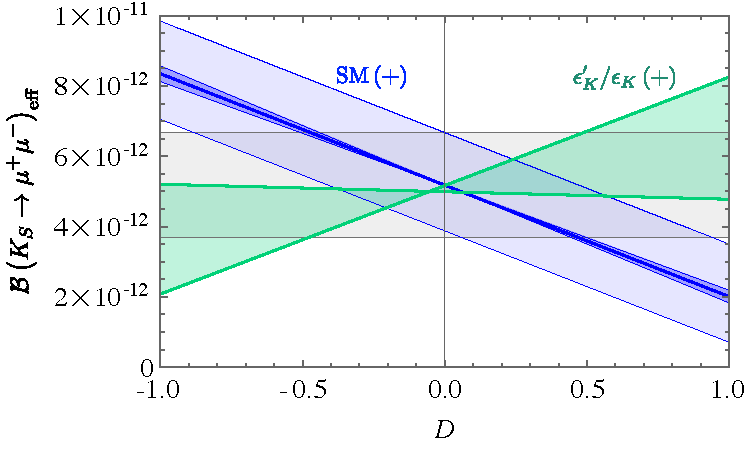
\includegraphics[width=0.46\textwidth]
{\main/section4/img/BrKSmumu_plus.pdf}
 ~~  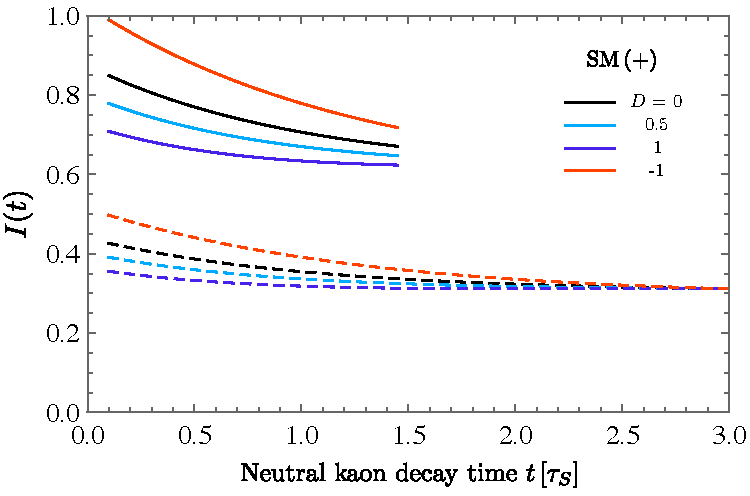
\includegraphics[width=0.42 \textwidth]{\main/section4/img/It_plus.pdf}
    \caption{ 
Left panel:  the effective branching ratios of Eq.~\eqref{eq:effBR} as function of dilution, $D$, Eq. \eqref{eq:DforK}, with blue band denoting the 
SM prediction, and the green band the new physics model that can explain the
$\varepsilon' /\varepsilon$ discrepancy \cite{Buras:2015yba,Kitahara:2016nld} (based on a lattice result \cite{Bai:2015nea}).
% is represented by the blue band. 
The gray band gives the SM prediction for zero dilution, 
%represents $\mathcal{B}(K_S \to \mu^+ \mu^-)_{\rm SM} $ in 
Eq.~\eqref{eq:KSmumu:SM}.
%A )   predicts  the green band.
%
Right panel: the $K \to \mu^+ \mu^- $  time distributions in the SM for several choices of $D$.  
%which are normalized by 
    The $D=0$ decay intensity is normalized, either over the interval $0.1 \tau_S$ to $1.45 \tau_S$ (solid lines) or $0.1 \tau_S$ to $3 \tau_S$ (dashed lines).
    Positive sign of $A^{\mu}_{L \gamma \gamma}$ is assumed in Eq.~\eqref{eq:ALgammagamma}.
    A detailed explanation and results for the negative sign of $A^{\mu}_{L \gamma \gamma}$ are given in Ref.~\cite{DAmbrosio:2017klp}.
}
\label{fig:time_distribution}
\end{figure}



\subsection{$K_S \to  \mu^+ \mu^- \gamma $, ~$K_S \to \mu^+ \mu^- e^+ e^-$  ~and ~$K_S \to \mu^+ \mu^- \mu^+ \mu^-$}


To improve the LD determination of $\mathcal{B}(K_S \to \mu^+ \mu^-)$, it is important  to measure $K_S \to  \mu^+ \mu^- \gamma $, $K_S \to \mu^+ \mu^- e^+ e^-$  and $K_S \to \mu^+ \mu^- \mu^+ \mu^-$.
These channels are at reach for \td{check:} LHCb \upgradetwo
%a high intensity machine 
and thus may give necessary LD  information needed for a better control of $K_{L}\rightarrow \mu^+ \mu^-$. 
These four body decays have a peculiar feature: similarly to $K_{S,L}\rightarrow \pi ^+ \pi ^- e^+ e^- $ \cite{Cirigliano:2011ny},
the two different helicity amplitudes interfere. 
One can then measure the sign of $ K_{L} \rightarrow \gamma ^\ast \gamma ^\ast \rightarrow  \ell^+ \ell^- \ell^+ \ell^-$  by studying  the time interference between $K_{S}$ and $ K_{L}$, which has a decay length	$2 \Gamma_S$ \cite{DAmbrosio:2013qmd}.

The 
%chiral 
ChPT prediction for $\mathcal{B}(K_S \to \gamma\gamma)$, experimentally confirmed, allows to make a  prediction for $\mathcal{B}(K_S \to  \mu ^+  \mu ^-  \gamma)=7.25\times 10^{-10}$; 
this value is increased by vector meson dominance (VMD) and unitarity corrections to
$\mathcal{B}(K_S \to \mu ^+  \mu^- \gamma  )=(1.45\pm 0.27)\times 10^{-9}$ \cite{Colangelo:2016ruc}.


\subsection{$K_S\to \pi^0 \ell^+ \ell^- $ and $K^\pm \to \pi^\pm \ell^+ \ell^- $}

\td{check:} At low dilepton mass squared, $q^2$,
%energy scale,
the dominant contribution to $K^\pm (K_{S}) \rightarrow \pi ^{\pm} 
(\pi ^{0})\ell ^{+}\ell ^{-}$ 
is due to a single virtual-photon exchange.
The resulting amplitude involves a vector form factor $V_i(z)$  ($i=\pm,S$),
which  can be decomposed in the general form up to ${\mathcal O}(p^6)$ in the chiral expansion as~\cite{DAmbrosio:1998gur}, 
\begin{equation}
  V_i(z) = a_i+ b_i z + V_i ^{\pi\pi}(z)\,, \quad z = q^2 / m_K^2\,,
  \quad \textrm{for}\quad i=\pm,S.
  \label{V_dec}
\end{equation}
Here the low energy constants (LECs), $a_i$ and $b_i$, parametrize the polynomial part of the amplitude, while the rescattering contribution $V_i^{\pi\pi}$ can be determined from fits to $K\to\pi\pi$ and $K\to\pi\pi\pi$ data (no $\Delta I=1/2$ contribution to $V_S^{\pi\pi}$). 
Chiral symmetry alone does not constrain the values of the LECs,
so instead, we consider the differential decay rate $d \Gamma / dz \propto |V_+(z)|^2$ 
as a means to extract $a_+$ and $b_+$ from experiment. 
The resulting fit to the decay spectra from all available high-statistics experiments is given in Table~\ref{tab:a+b+}.
The experimental size of the $b_{+}/a_{+}$ ratio 
exceeds the naive dimensional analysis estimate, calling  
for  large VMD. 

\begin{table}[t]
\renewcommand{\arraystretch}{1.3}
\centering
\caption{Fitted values of coefficients entering the vector form factor in Eq.~\eqref{V_dec}.}
\label{tab:a+b+}
\begin{tabular}{cccr}
%\toprule
\hline\hline
Channel & $a_+$ & $b_+$ & Reference \\
\hline
$ee$ & $-0.587\pm 0.010$ & $-0.655\pm 0.044$ & E865~\cite{Appel:1999yq}\\
$ee$ & $-0.578\pm 0.016$ & $-0.779\pm 0.066$ & NA48/2~\cite{Batley:2009aa}\\
$\mu\mu$ & $-0.575\pm 0.039$ & $-0.813\pm 0.145$ & NA48/2~\cite{Batley:2011zz}\\%\bottomrule
\hline\hline
\end{tabular}
\end{table}

The branching ratios of $K_S \to \pi^0 \ell^+ \ell^-$, on the other hand, are  approximately 
\begin{equation}
 \mathcal{B}(K_S \rightarrow \pi^0 e^+ e^-)   
   \approx     5 \times 10^{-9} \cdot a_S^2, \qquad  
   \mathcal{B}(K_S \rightarrow \pi^0 \mu ^+  \mu ^-)  
   \approx     1.2  \times 10^{-9}  \cdot  a_S^2,
\label{eq:BRKS}
\end{equation}
and   NA48, assuming just a VMD form factor, finds respectively \cite{Batley:2003mu,Batley:2004wg} 
 \begin{equation}
  | a_S|_{e e } = 1.06 ^{+0.26} _{-0.21} \pm 0.07, 
 \qquad
 |a_S|_{\mu \mu } = 1.54 ^{+0.40} _{-0.32} \pm 0.06.
\end{equation}
The uncertainty of $|a_S|_{\mu \mu }$ gives the dominant theoretical uncertainty in $K_L \to \pi^0 \mu^+ \mu^-$.
Therefore,
this measurement is a crucial piece of information required to establish the relative roles of indirect $\CP$ violation vs. direct $\CP$ violation  in $ K_L \rightarrow \pi^0 \mu ^+  \mu ^-$, in order to probe SD effects \cite{Mescia:2006jd}.
The LHCb \upgradetwo can reach a precision in $\mathcal{B}(K_S^0\to\pi^0\mu^+\mu^-)$  at the $10^{-10}$ level (see Fig. \ref{fig:KpzSens}), and, through an analysis of the differential decay rate, a $10\%$ statistical precision on the form factor term $|a_S|$ with free $b_S$~\cite{kaon_paper}.

\begin{figure}[t]
\begin{center}
\vspace{-0.2cm}
\includegraphics[scale=0.8]{\main/section4/img/sensitPARTIAL.pdf}
\vspace{-0.1cm}
\caption{Projected LHCb reach for $\mathcal{B}(K_S^0\to\pi^0\mu^+\mu^-)$ as a function of the integrated luminosity times trigger efficiency (which is expected to be ${\mathcal O}(1)$ in LHCb \upgradetwo. Figure adapted from Ref. \cite{Chobanova:2195218}.}
\label{fig:KpzSens}
\vspace{-1cm}
\end{center}
\end{figure}

\subsubsection{Lepton flavor universality violation in $K^\pm \to \pi^\pm \ell^+\ell^-$}
The coefficients $a_+$ and $b_+$  can be used to test for Lepton flavor universality violation (LFUV). 
 If lepton flavour universality applies each of the two coefficients, averaged over different experiments, have to be equal for the $ee$ and $\mu\mu$ channels. Within errors this is indeed the case, see Table \ref{tab:a+b+}.  Since the SM interactions are lepton flavour universal, deviations from zero in differences, such as $a_+^{\mu\mu} - a_+^{ee}$, would  be a sign of NP. 
 %The corresponding effect would be necessarily short distance. 
Such test are especially interesting in view of the $B$-physics anomalies (see ~\ref{secBanom}), with rare kaon decays providing a complementary role in testing the NP explanations.  Our analysis~\cite{Crivellin:2016vjc} is based on the observation that at low energy scales, $\mu \ll m_{t,b,c}$, 
the strangeness-changing transitions are described in terms of the effective Lagrangian~\cite{Cirigliano:2011ny}
\begin{equation}
\label{Lagr_K}
  {\cal L}_\text{eff}^{|\Delta S|=1} = 
  - \frac{G_F}{\sqrt{2}} V_{ud}V_{us}^* \sum_{i} C_i(\mu) Q_i(\mu) + \text{h.c.} \,,
\end{equation}
which contains semileptonic operators
\begin{align}\label{eq:Q11-12}
Q_{7V} =   \left[\bar s \gamma^\mu (1 - \gamma_5) d \right]
\sum_{\ell=e,\mu} \left[\bar{\ell} \gamma_\mu  \ell \right], \quad \mbox{and} \quad
Q_{7A} = \left[\bar s \gamma^\mu (1 - \gamma_5) d \right]
\sum_{\ell=e,\mu}  \left[\bar{\ell} \gamma_\mu \gamma_5 \ell \right], 
\end{align}
that are the $s\to d$ analogues of the $b\to s$ operators, $Q_{9,10}^B$.  In the framework of minimal flavour violation (MFV), the Wilson coefficients of the two sectors are correlated. We use this feature to convert knowledge of $C_{7V,7A}$ into bounds on $C_{9,10}^B$.  

 To convert the allowed range on $a_+^\text{NP}$ into a corresponding range in the Wilson coefficients $C_{7V}^{\ell\ell}$, we make use of the ${\mathcal O}(p^2)$ chiral realization of the $SU(3)_L$ current
\begin{equation}
  \bar{s}\gamma^\mu(1-\gamma_5)d \leftrightarrow i f_\pi^2 (U\partial^\mu U^\dagger)_{23}\,, 
  \qquad U = U(\pi,K,\eta)\,, 
  \label{bosonize}
\end{equation}
to obtain 
\begin{equation}
 a_+^\text{NP}=\frac{2\pi\sqrt{2}}{\alpha}V_{ud}V_{us}^*C_{7V}^\text{NP}\,.
 \label{aNP}
\end{equation}
Contributions due to NP in $K^+ \to \pi^+ \ell^+\ell^-$ can then be probed by considering the difference between the two channels
\begin{equation}
\label{limit_Kp}
 C_{7V}^{\mu\mu}-C_{7V}^{ee}=\alpha\frac{a_+^{\mu\mu}-a_+^{ee}}{2\pi\sqrt{2}V_{ud}V_{us}^*}\,.
\end{equation}
Assuming MFV, this can be converted into a constraint on the NP contribution to $C_9^B$,
\begin{equation}
\label{C_charged}
 C_{9}^{B,\mu\mu}-C_{9}^{B,ee}=-\frac{a_+^{\mu\mu}-a_+^{ee}}{\sqrt{2}V_{td}V_{ts}^*}\approx -19\pm 79\,,
\end{equation}
where we have averaged over the two electron experiments listed in Table~\ref{tab:a+b+}.

The determination of $a_+^{\mu\mu}-a_+^{ee}$ needs to be improved by an ${\mathcal O}(10)$ factor in order to probe the parameter space relevant for the $B$-anomalies, which require Wilson coefficients $C_{9,10}^B={\mathcal O}(1)$~\cite{Descotes-Genon:2015uva}. Improvements of this size may be possible at NA62, especially for the experimentally cleaner dimuon mode which currently has the larger uncertainty. 






\subsection{$K_S\to \pi^+ \pi^- e^+ e^-$}
The $  K_S \rightarrow \pi^+ \pi^- e^+ e^- $ decays 
can be interesting, if one can test  beyond the dominant bremsstrahlung contribution, 
performing  ChPT tests. \td{check:} In principle, 
%NP  and 
$\CP$ violation is also of interest for NP searches.
%, in principle, interesting to investigate. 
So far,  NA48   has, using 676 events, obtained a measurement
$\mathcal{B}(  K_S \rightarrow \pi^+ \pi^- e^+ e^- )=(4.79\pm 0.15)\times 10^{-5}$, 	 		
\cite{PDG2018} 
to be compared with the theoretical prediction \cite{Cappiello:2017ilv}
\begin{align}
\mathcal{B}(K_S\to \pi^+\pi^-e^+e^-)=\underbrace{4.74\cdot 10^{-5}}_{\text{Brems.}}+\underbrace{4.39\cdot 10^{-8}}_{\text{Int.}}+\underbrace{1.33\cdot 10^{-10}}_{\text{DE}}~.
\end{align}
Similarly, one can predict for the dimuon channel, 
%that
\begin{align}
\mathcal{B}(K_S\to \pi^+\pi^-\mu^+\mu^-)=\underbrace{4.17\cdot 10^{-14}}_{\text{Brems.}}+\underbrace{4.98\cdot 10^{-15}}_{\text{Int.}}+\underbrace{2.17\cdot 10^{-16}}_{\text{DE}}~.
\end{align}


\subsection{LFV modes}

Modes with LFV, such as $K \to (n \pi) \mu^\pm e^\mp$, provide null tests of the SM. Sizable BSM contributions to such processes have renew theoretical motivation because of the hints for LFUV
%Universality Violation (LUV) 
in $B \to K^{(\ast)} \ell^\pm \ell^\mp$ processes. Both types of processes can arise from NP contributions to the product of the two neutral currents, composed of the down-type quarks and charged leptons. The only difference between the two is the strength of the flavour couplings involved.
Using general EFT arguments, the amount of LFUV hinted at in $B \to K^{(\ast)} \ell^\pm \ell^\mp$ decays, generically imply $B \to K^{(\ast)}$ LFV rates of the order of $10^{-8}$ \cite{Glashow:2014iga}. (More quantitative estimates require introduction of flavour models \cite{Guadagnoli:2015nra,Boucenna:2015raa,Celis:2015ara,Alonso:2015sja,Gripaios:2015gra,Crivellin:2016vjc,Becirevic:2016zri,Becirevic:2016oho,Hiller:2016kry,Becirevic:2017jtw,Buttazzo:2017ixm,King:2017anf,Bordone:2018nbg}.) 

As discussed in Ref. \cite{Borsato:2018tcz}, such arguments can be extended to $K \to (\pi) \mu^\pm e^\mp$, with fairly general assumptions on different flavour couplings involved. Expected rates can be as large as $10^{-10} - 10^{-13}$ for the $K_L \to \mu^\pm e^\mp$ mode and a factor of $\sim 100$ smaller for the $K^+ \to \pi^+ \mu^\pm e^\mp$ one. Taking into account the suppression mechanisms at play, such ``large'' rates are a non-trivial finding. The relatively wide predicted ranges are due to the inherent model dependence, especially in the choice of the leptonic coupling and of the overall scale of the new interaction, typically between $5$ and $15$ TeV \cite{Borsato:2018tcz}. On the experimental side, the limits on $K \to (\pi) \mu^\pm e^\mp$ modes are, somewhat surprisingly, decade-old
\begin{eqnarray}
\label{eq:limits}
\begin{tabular}{clcl}
$\mathcal B(K_L \to e^\pm \mu^\mp) < 4.7 \times 10^{-12}$ & \hspace{-0.3cm}\cite{Ambrose:1998us}~, &~~~~
$\mathcal B(K_L \to \pi^0 e^\pm \mu^\mp) < 7.6 \times 10^{-11}$ & \hspace{-0.3cm}\cite{Abouzaid:2007aa}~,\\
[0.1cm]
$\mathcal B(K^+ \to \pi^+ e^- \mu^+) < 1.3 \times 10^{-11}$ & \hspace{-0.3cm}\cite{Sher:2005sp}~, &~~~~
$\mathcal B(K^+ \to \pi^+ e^+ \mu^-) < 5.2 \times 10^{-10}$ & \hspace{-0.3cm}\cite{Appel:2000tc}~.\\
\end{tabular}
\end{eqnarray}
These modes can be profitably pursued at the upgraded LHCb, which will benefit from huge yields. %In fact, starting from a total $K^\pm$ cross section of 630~mb, and taking into account that $\sim 22\%$ of kaons are in the pseudorapidity acceptance of LHCb, one can estimate a $K^\pm$ cross-section as large as $1.4\times 10^{14}$~fb \cite{Borsato:2018tcz}. 
Ref. \cite{Borsato:2018tcz} presented a feasibility study for the modes in Eq. (\ref{eq:limits}), taking $K^+ \to  \pi^+ \mu^\pm e^\mp$ as a benchmark. The expected reach is displayed in Fig. \ref{fig:K_LFV} as a function of the integrated luminosity and for different scenarios of detector performance. This shows that LHCb \upgradetwo could update some of the existing limits, a result that per se already makes these searches promising. 
Even more interestingly, LHCb \upgradetwo 
 could probe part of the parameter space for LFV kaon decays suggested by the $B$-physics anomalies. This conclusion in turn calls attention to other running and upcoming facilities, including Belle-II, NA62~\cite{NA62:2312430}, as well as the newly proposed TauFV~\cite{PBCTalk}. %NA62 is a dedicated $K^+$ experiment with exquisite light-lepton identification capabilities, and as such is expected to be very competitive, at least on charged modes. TauFV~\cite{PBCTalk} in turn may benefit from no less than $O(10^{19})$ kaons in a decay volume of a similar size to LHCb's and with a similar detector layout. 
Dedicated sensitivity studies for these facilities are required in order to make more quantitative statements. Yet, the experimental outlook for all these modes is certainly promising.

\begin{figure}[t]
\begin{center}
\vspace{-0.2cm}
\includegraphics[scale=0.5]{\main/section4/img/BRvslumi_ptscan.pdf}
\vspace{-0.1cm}
\caption{Expected reach for $K^+\to \pi^+\mu^\pm e^\mp$ as a function of the integrated luminosity with 13~TeV $pp$ collisions based on a fast simulation of LHCb. Different scenarios in terms of PID performance and $p_{\rm T}$ thresholds of the $\pi^+$ and $e^{\pm}$ candidates are shown. Combinatorial background is neglected in the study. Figure adapted from Ref. \cite{Borsato:2018tcz}.}
\label{fig:K_LFV}
\vspace{-1cm}
\end{center}
\end{figure}

\subsection{Hyperons at HL-LHC}

The LHCb can contribute significantly to the strangeness-physics program with measurements of hyperon decays. There is vast room for improvement in this sector as most of the data for the SM, both nonleptonic and semileptonic decays, is about 40 years old, and many of the rare decays sensitive to SD physics have not even been searched for. 
An exploratory study of the LHCb's potential in hyperon physics was presented in~\cite{Junior:2018odx}; here we summarize the main conclusions. 

Current experimental data on the semileptonic hyperon decays $\Lambda\to p\mu^-\bar\nu$, $\Xi^-\to\Lambda\mu^-\bar\nu$ and $\Xi^-\to\Sigma^0\mu^-\bar\nu$ is quite poor, with relative uncertainties in the range of 20\%-100\%. These decay modes can be partially reconstructed at the LHCb, where the kinematic distributions allow one to discriminate from the peaking backgrounds of $\Lambda\to p\pi^-$ and $\Xi^-\to\Lambda\pi^-$. Besides testing lepton-universality by comparing with the semi-electronic modes, these decays are sensitive to BSM scalar and tensor currents~\cite{Chang:2014iba}. 
%Finally, i
If percent precision is achieved in the measurement of semi-muonic branching fractions, they could contribute to a better determination of the CKM matrix element $|V_{us}|$ from hyperon decays~\cite{Cabibbo:2003cu,Cabibbo:2003ea}. 

A golden mode among the rare hyperon decays is $\Sigma^+\to p \mu^+\mu^-$, to which LHCb recently contributed with an evidence for the decay at 4.1$\sigma$ and a di-muon invariant distribution consistent with the SM~\cite{Aaij:2017ddf}, thus challenging the HyperCP anomaly~\cite{Park:2005eka}. With dedicated triggers and the upgraded LHCb detector in the HL phase about a thousand events per year of data-taking could be measured, which will allow to measure angular distributions or direct $\CP$ asymmetries that have been shown to be sensitive to SD physics~\cite{Meinel:2017ggx,He:2018yzu}. The equivalent channel with lepton number violation, $\Sigma\to\bar{p}\mu^+\mu^+$ can also be searched for, with potential sensitivities at the $10^{-9}$ level. Other $\Delta S=1$ semileptonic rare hyperon decays, except those of the $\Omega^-$ (which will be produced at a rate similar to that of a $B$-meson), must have electrons in the final state due to phase space. Sensitivity to $\mathcal B(\Sigma^+\to p e^+e^-)\sim 10^{-6}$ should be accessible at LHCb, whereas other modes like $\Lambda\to p \pi^- e^+e^-$ suffer from low electron reconstruction efficiency. More exotic modes, probing baryon-number violation, lepton-flavor violation, or $\Delta S=2$, can also be measured with projected sensitivities improving by orders of magnitude the current limits~\cite{Junior:2018odx}. 
Radiative decays such as $\Lambda \to p \pi \gamma$ are also accessible to LHCb.


\end{document}
